\documentclass{article}


% if you need to pass options to natbib, use, e.g.:
%     \PassOptionsToPackage{numbers, compress}{natbib}
% before loading neurips_2023


% ready for submission
\usepackage{neurips_2023}


% to compile a preprint version, e.g., for submission to arXiv, add add the
% [preprint] option:
%     \usepackage[preprint]{neurips_2023}


% to compile a camera-ready version, add the [final] option, e.g.:
%     \usepackage[final]{neurips_2023}


% to avoid loading the natbib package, add option nonatbib:
%    \usepackage[nonatbib]{neurips_2023}


\usepackage[utf8]{inputenc} % allow utf-8 input
\usepackage[T1]{fontenc}    % use 8-bit T1 fonts
\usepackage{hyperref}       % hyperlinks
\usepackage{url}            % simple URL typesetting
\usepackage{booktabs}       % professional-quality tables
\usepackage{amsfonts}       % blackboard math symbols
\usepackage{nicefrac}       % compact symbols for 1/2, etc.
\usepackage{microtype}      % microtypography
\usepackage{xcolor}         % colors
\usepackage{graphicx}
\usepackage{subcaption}

\title{Keypoint Detection}


% The \author macro works with any number of authors. There are two commands
% used to separate the names and addresses of multiple authors: \And and \AND.
%
% Using \And between authors leaves it to LaTeX to determine where to break the
% lines. Using \AND forces a line break at that point. So, if LaTeX puts 3 of 4
% authors names on the first line, and the last on the second line, try using
% \AND instead of \And before the third author name.

  % examples of more authors
  % \And
  % Coauthor \\
  % Affiliation \\
  % Address \\
  % \texttt{email} \\
  % \AND
  % Coauthor \\
  % Affiliation \\
  % Address \\
  % \texttt{email} \\
  % \And
  % Coauthor \\
  % Affiliation \\
  % Address \\
  % \texttt{email} \\
  % \And
  % Coauthor \\
  % Affiliation \\
  % Address \\
  % \texttt{email} \\

\author{
}





\begin{document}


\maketitle

\section{\fontsize{12}{14}\selectfont Abstract}

Our interest lies in addressing the human pose estimation problem, emphasizing the acquisition of dependable high-resolution representations. Unlike many current approaches that reconstruct high-resolution representations from low-resolution counterparts generated by a high-to-low resolution network, our  proposed network preserves high-resolution representations throughout the entire process.

In our approach, we initiate the network with a high-resolution subnetwork as the initial stage. Subsequently, we systematically introduce additional stages, each incorporating high-to-low resolution subnetworks. These subnetworks operate in parallel, and through a series of repeated multi-scale fusions, information is exchanged among the different resolution representations. This iterative fusion process enhances the richness of high-resolution representations, potentially leading to more accurate and spatially precise predictions of key points. Our empirical findings substantiate the efficacy of this network architecture, showcasing superior performance in pose estimation when evaluated on the COCO dataset.


\section{\fontsize{12}{14}\selectfont Introduction}

Improper posture can lead to persistent pain, discomfort, diminished productivity, and a decline in overall quality of life. The project's focus lies in identifying key points on the human body with the goal of developing a system for posture detection and correction during diverse activities like sitting or exercising. Exam monitoring is another application that can be developed but we are specifically concerned about exercise. By concentrating on a targeted set of key points, the project seeks to track and discern changes in humans' posture movements, addressing the broader issue of poor posture and its associated consequences.

Introduced an architecture called High Resolution Net (HRNet), designed to preserve high-resolution representations throughout the entire process. The network offers two advantages over commonly used networks [1, 2, 3, 4] for pose estimation. Firstly, unlike most existing solutions, our approach connects high-to-low resolution subnetworks in parallel instead of in series. This enables us to maintain high resolution rather than recovering it through a low-to-high process, potentially leading to a more spatially precise predicted heatmap. Secondly, while many fusion schemes in existing methods aggregate low-level and high-level representations, we employ repeated multiscale fusions to enhance high-resolution representations using low-resolution representations of the same depth and similar level, and vice versa. This results in rich high-resolution representations for pose estimation, potentially making our predicted heatmap more accurate.

The unique contribution of this project lies in its innovative approach to detecting and correcting improper posture through the introduction of keypoint detection and correction algorithms. Unlike conventional methods that may focus solely on monitoring posture without offering corrective measures, our system not only identifies key points on the human body during diverse activities such as sitting or exercising but also provides real-time suggestions for correcting posture based on these keypoint analyses. This proactive approach aims to address the root causes of poor posture and prevent associated discomfort and pain. This combination of keypoint detection, correction suggestions, and advanced architectural design sets our project apart, offering a comprehensive solution to the pervasive issue of improper posture and its detrimental effects on overall well-being.


\section{\fontsize{12}{14}\selectfont Related Work}
Some of the current trends and different frameworks that are dealing with key-point detection are:

\textbf{EfficientPose}

This framework incorporates efficiency as a pivotal parameter. The architecture is composed of two integral elements: an efficiency backbone and an efficiency head. The methodology employed in the paper [5] involves the implementation of a differentiable neural architecture, serving as the backbone for efficiency by diminishing computational requirements while maintaining backbone accuracy. Within the efficiency head, specific operations are streamlined to enhance the ultimate prediction. Notably, this model operates with a computational load of only 2 GFLOPS, a notable reduction compared to HRNet's 9.5 GFLOPS.

\textbf{HRNet}

This architecture preserves a high-resolution image from the initial stages. The model gathers information across various resolutions, incorporating a high-resolution fusion module that effectively amalgamates features extracted from both high and low-resolution images, thereby enhancing the model's precision.

\textbf{CentreNet}

The primary objective in introducing this framework is precise object localization. A key feature is the incorporation of the concept of "center-ness" to enhance prediction accuracy. This parameter gauges the distance of an object from the center, effectively filtering out inaccurate positives and refining prediction precision. CentreNet employs diverse backbone networks, including ResNet or Hourglass, to support its operations.

\textbf{OpenPose}

This model exhibits the capability to identify numerous individuals within a provided image or video. Its modular architecture empowers users to tailor its configuration to suit their specific requirements.

\textbf{Integrated Human Pose Regression} 

This approach emphasizes the significance of encoding spatial interconnections among distinct body elements. Through comprehensive pose regression, it gains insights into the holistic structure of the human body. The integration process mitigates ambiguity in pose estimation.

\textbf{Stacked hourglass networks for human pose estimation} 
Utilizing convolutional neural networks (ConvNets), the architecture adopts a stacked hourglass design, enabling iterative bottom-up and top-down inference across various scales. This design promotes the extraction of hierarchical features, allowing for a comprehensive understanding of posture-related information. The convolutional nature of the network ensures effective processing of spatial information, while the stacked hourglass configuration enhances the model's ability to capture intricate details, contributing to the system's robustness in posture detection and correction.




\section{\fontsize{12}{14}\selectfont System Design}
\subsection{Overview}
The project focuses on implementing real-time human pose estimation using the HRNet model on a Raspberry Pi 4. The system's primary objective is to detect 17 keypoints on the human body, assess the user's posture during exercises, and provide corrective suggestions. The solution involves training an HRNet model, optimizing it for deployment on the Raspberry Pi, and incorporating a real-time feedback mechanism.

\subsection{Architecture Overview}
The proposed system architecture consists of key components: data preprocessing, the HRNet pose estimation model, and a real-time feedback module (to be worked on as a part of future application).

\subsection{Data Preprocessing}
In the data preprocessing pipeline, two crucial steps are undertaken to optimize image and label data for effective utilization in the posture detection and correction model. Firstly, for image data, a standardized resolution is enforced by resizing each image to a dimension of 384x288 pixels. Subsequently, the pixel values are normalized to a scale ranging from 0 to 1. This normalization process ensures consistency in data representation, enhancing the model's ability to learn and generalize across diverse images. Moreover, the normalization step employs specific mean and standard deviation values derived from the ImageNet dataset, where the mean is set to [0.485, 0.456, 0.406] and the standard deviation is [0.229, 0.224, 0.225]. This normalization aligns the image data with the characteristics of the ImageNet dataset, promoting better convergence during training.

Secondly, in the context of label data preprocessing, a key step involves creating binary masks for annotated keypoints. Each keypoint is surrounded by a circle with a fixed radius of 6 pixels, assigning a pixel value of 1 within the circle and 0 elsewhere. This process transforms the annotation into a binary representation, facilitating the model's understanding of keypoint localization. The creation of these binary masks for all 17 annotated keypoints contributes to the generation of precise ground truth labels for training the posture detection model. The incorporation of such meticulous label preprocessing ensures that the model can effectively learn the spatial relationships and positional information of keypoints during the training phase, ultimately enhancing its accuracy in detecting and correcting improper postures across various activities, such as sitting or exercising. The combination of image and label data preprocessing sets a solid foundation for the robust performance of the posture detection and correction system.


\subsection{HRNet Model}
The chosen architecture for this posture detection and correction system is HRNet, which employs stacked parallel sub-networks for multi-resolution feature extraction. The decision to opt for HRNet is motivated by its exceptional ability to preserve high-resolution representations throughout the network, crucial for accurate keypoint localization. The parallel sub-networks within HRNet facilitate the capture of both fine-grained and high-level features, thereby enhancing the overall accuracy of the model. Additionally, HRNet employs a multi-scale fusion process, allowing the simultaneous maintenance of high-resolution and low-resolution features, contributing to effective feature preservation. To cater to lightweight applications, a Simple HRNet implementation is chosen, making it ideal for embedded systems. However, it's worth noting that a Deep HRNet may incur memory overhead, particularly on 8GB microprocessors, necessitating a thoughtful consideration of resource constraints in deployment scenarios.

\subsection{Converting PyTorch Model to TensorFlow Lite for Raspberry Pi Implementation}
In the process of transitioning the posture detection and correction model from PyTorch to TensorFlow Lite for deployment on a Raspberry Pi embedded system, a systematic flowchart is adopted. The initial step involves converting the PyTorch model to the Open Neural Network Exchange (ONNX) format, creating an intermediate representation that is compatible with various frameworks. Subsequently, the ONNX model is transformed into a TensorFlow model, ensuring seamless integration into the TensorFlow ecosystem. Finally, the TensorFlow model is further converted to TensorFlow Lite (TFLite), optimizing it for deployment on resource-constrained environments such as the Raspberry Pi. This comprehensive flowchart ensures a smooth and interoperable transition between PyTorch and TensorFlow Lite, allowing the posture detection and correction system to efficiently run on embedded systems with limited computational resources.

\subsection{Installing Ubuntu on Raspberry Pi for Posture Detection System}
In the initial phase of our project implementation, we opted to install Ubuntu on the Raspberry Pi, a departure from the standard Raspbian OS, primarily for its enhanced compatibility with a broader range of software packages and development tools. Utilizing the Raspberry Pi Imager, we downloaded the Ubuntu 64-bit operating system, tailored for better performance on the Raspberry Pi's ARM architecture. This choice aligns with our project's computational requirements, ensuring seamless integration with machine learning libraries and frameworks. After downloading, the Ubuntu OS was burned onto the SD card using the Raspberry Pi Imager.

Upon successful installation, we set up the Raspberry Pi system with a monitor, keyboard, and mouse, providing a user-friendly interface for configuration and testing. The Ubuntu environment was chosen for its user-friendly interface and extensive community support, facilitating system setup and subsequent developments.

To integrate the posture detection model with real-time video feed, we employed OpenCV and configured the Raspberry Pi camera module. Through Python scripts, we programmed the camera to capture a continuous feed and implemented the posture detection algorithm using the TensorFlow Lite model. This integration marks a critical step in our project, as it enables real-world testing of the posture detection and correction system in varied environments. The successful implementation of Ubuntu on the Raspberry Pi lays the foundation for robust and efficient deployment of our posture detection solution, showcasing its adaptability and performance on an embedded system.

\subsection{Deploying Simple HRNet on Raspberry Pi for Live Demo}
In this phase of our project, we executed the Simple HRNet code on the Raspberry Pi, integrating the posture detection model into the Ubuntu environment. The implementation includes capturing a live demo video using the Raspberry Pi camera module to facilitate real-time testing and evaluation of the posture detection system. This deployment on the Raspberry Pi underscores the practical applicability and efficiency of the Simple HRNet architecture in a resource-constrained embedded environment, showcasing its potential for real-world posture detection and correction applications.


\subsection{Future Work: Algorithm Development for Posture Correction Feedback}
A crucial avenue for future work involves the development of algorithms that provide real-time corrective suggestions based on deviations from correct poses. This enhancement aims to offer users immediate visual or auditory feedback, guiding them towards adopting proper postures during activities such as sitting or exercising. Implementing intelligent feedback mechanisms will not only bolster the effectiveness of the posture detection system but also contribute to the user's proactive engagement in maintaining optimal postural habits.

\subsection{Challenges Faced During Model Conversion and Deployment}
The process of converting our PyTorch model to ONNX presented a significant challenge related to data parallelism. In the original model trained with multiple GPUs, data parallelism was employed, where each GPU loaded different batches of data for the same model simultaneously. However, during the conversion to ONNX, this approach led to complications, prompting the removal of data parallelism from the model. Data parallelism, in the context of multi-GPU training, involves each GPU processing distinct batches of data for a shared model, aiming to expedite training.

Furthermore, an interoperability issue arose due to the use of dots in module names by PyTorch, a format not supported by TensorFlow. To address this, a necessary adjustment was made by replacing dots with underscores, ensuring compatibility during the conversion process.

Another notable challenge pertained to compatibility issues with different operating systems during the installation procedure. The diverse requirements and dependencies across operating systems led to unforeseen complications, demanding meticulous troubleshooting to achieve seamless integration. This underscored the importance of thorough compatibility checks and adaptations to accommodate variations in the deployment environment.

In overcoming these challenges, the project team demonstrated resilience and adaptability, ensuring the successful conversion and deployment of the posture detection model. The removal of data parallelism, adjustment of module naming conventions, and diligent troubleshooting for OS compatibility not only resolved these issues but also enriched the project team's expertise in navigating the intricacies of model conversion and deployment processes. These experiences contribute valuable insights into the complexities inherent in deploying machine learning models across different frameworks and systems.


\begin{figure}
  \centering
  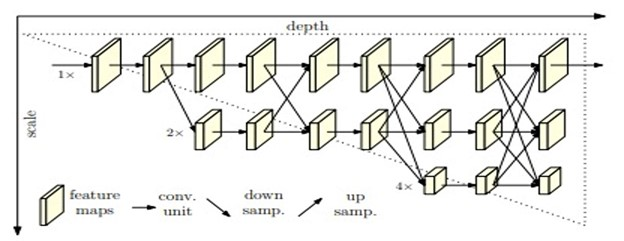
\includegraphics[width=\textwidth]{Picture.jpg}
  \caption{Multi-scale feature fusion HRNet}
  \label{fig1}
\end{figure}

\begin{figure}
  \centering
  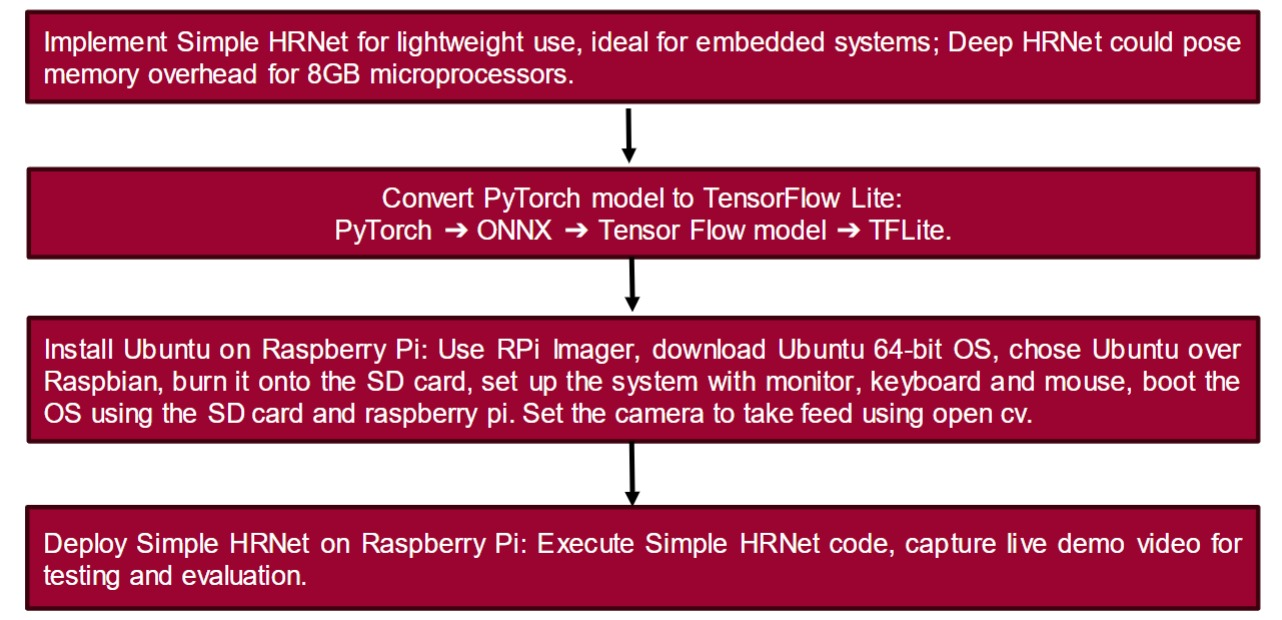
\includegraphics[width=\textwidth]{flow_chart.jpg}
  \caption{Flow Diagram of the system design}
  \label{fig2}
\end{figure}




\section{\fontsize{12}{14}\selectfont Evaluation Approach}

In the realm of computer vision, particularly in the domain of human pose estimation, the evaluation approach is a critical aspect that determines the efficacy and reliability of the deployed model. The success of a model in accurately predicting keypoints on human bodies has profound implications, ranging from sports analytics to healthcare applications. In this context, the evaluation approach for the Human Pose Estimation using the HRNet model involves a combination of custom data collection, model training on the COCO dataset, and the utilization of the  Average Precision (AP) score as the primary evaluation metric.

\subsection{Data Collection:}
The foundation of any machine learning model lies in the quality and relevance of the data it is trained on. In this work, custom data has been collected, featuring pictures of project teammates for inference. This personalized dataset introduces a real-world element, ensuring that the model is exposed to diverse scenarios and individuals. The COCO dataset, a widely accepted benchmark for human pose estimation, is incorporated into the training process. Its inclusion provides the model with a comprehensive understanding of human poses, thanks to the meticulously annotated 17 keypoints for each image.

\subsection{Model Selection and Training:}
The HRNet model has been chosen for its outstanding performance in human pose estimation tasks. Unlike traditional approaches that downsample the input image, HRNet maintains high-resolution representations throughout the network, capturing intricate details essential for accurate keypoint localization. The training process involves leveraging the COCO dataset to fine-tune the model's parameters, enabling it to generalize well to various human poses. Training for 10 epochs strikes a balance between learning from the data and preventing overfitting.

\subsection{Evaluation Metric:}
In the rigorous evaluation of our posture detection model, the Average Precision (AP) score emerges as a pivotal metric for its ability to comprehensively gauge the model's effectiveness in precisely localizing keypoints. AP strikes a balance between precision and recall, offering a nuanced understanding of the model's capabilities in identifying key body points. This metric is particularly apt for pose estimation tasks where spatial accuracy is paramount.

Upon assessing the performance of both simple HRNet (AP=0.817) and deep HRNet (AP=0.925), a noteworthy observation surfaced: the output from the basic HRNet was nearly identical and highly comparable to that of the deep HRNet. While the deep HRNet exhibited a marginally higher AP value, the computational constraints posed by its memory overhead raised practical concerns, especially in the context of deploying the model on embedded systems like the Raspberry Pi. Despite the slightly superior AP of the deep HRNet, the decision was made to opt for the simple HRNet for deployment. This strategic choice stems from the consideration of computational efficiency and resource limitations inherent to embedded systems. The AP of the simple HRNet, while marginally lower, remains impressive at 0.817, making it a pragmatic and resource-conscious selection for the Raspberry Pi.

Therefore, the deployment of the simple HRNet on the Raspberry Pi aligns with our goal of balancing performance and computational constraints. The model's AP of 0.817 underscores its efficacy in posture detection, making it a suitable choice for real-time applications on embedded platforms. This decision ensures that our posture detection and correction system maintains a high level of accuracy while optimizing for the inherent limitations of the Raspberry Pi's computational resources.


\subsection{Custom Data Testing:}
Beyond quantitative metrics, the model is subjected to real-world testing using custom data. This step is crucial in validating the model's generalization to scenarios beyond the training data. The ability of the model to accurately detect keypoints in the 1st and 4th pictures, indicate the importance of multi-scale feature fusion mechanism employed in the HRNet model.



\section{Results}
The evaluation of the posture detection model involved a thorough analysis of its performance across training epochs. Graphs tracking the Average Precision (AP) score over time provided a visual representation of the model's convergence and stability. An increasing AP score throughout the epochs signified the model's continuous refinement, adapting to the complexities within the dataset. This iterative learning approach ensured the development of a robust representation of human poses.

Notably, the output from the basic HRNet, with an mAP of 0.817, demonstrated a performance nearly identical and highly comparable to the deep HRNet with an mAP of 0.925. Despite the slightly higher mAP of the deep HRNet, practical considerations led to the decision to deploy the simple HRNet on the Raspberry Pi. The conversion from PyTorch to TensorFlow Lite exhibited no performance degradation, maintaining the model's accuracy during the transition.

The model showcased proficiency in predicting keypoints, even in scenarios involving occlusion. This capability is crucial for real-world applications where partial visibility of body parts may occur. Additionally, the TensorFlow Lite model demonstrated satisfactory frames per second (fps) for inference on the Raspberry Pi, even when processing low-resolution images. This efficiency is pivotal for real-time applications, ensuring the system's responsiveness in diverse environments.

The observed robust performance in both keypoint prediction under occlusion and satisfactory fps on the Raspberry Pi can be attributed to the resilience of the COCO dataset. The diverse and extensive annotations within the COCO dataset contribute to the model's adaptability, enabling accurate predictions across various scenarios. This dataset's impact on the model's generalization capability is evident in its ability to handle challenging conditions, making it a valuable resource for training models in real-world applications.

In summary, the posture detection model, particularly when deployed with the simple HRNet architecture on the Raspberry Pi, demonstrated commendable accuracy and efficiency. The evaluation metrics, coupled with real-world testing scenarios, affirm the model's viability for practical deployment in environments where real-time posture detection and correction are crucial. These results not only validate the effectiveness of the chosen architecture and dataset but also showcase the adaptability of the system for embedded applications, such as those encountered in the deployment on the Raspberry Pi.

\begin{figure}
  \centering
  \begin{subfigure}[b]{0.4\textwidth}
    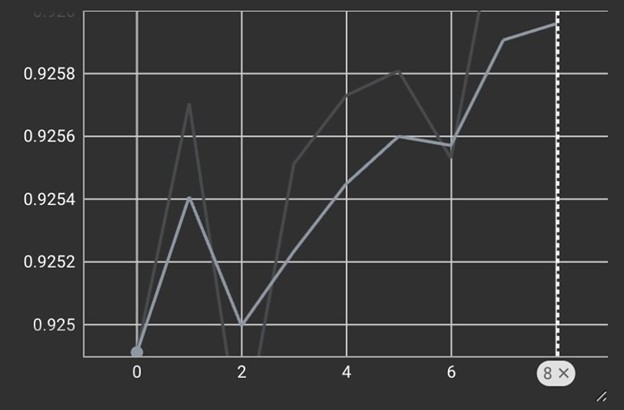
\includegraphics[width=\textwidth]{Picture1.jpg}
    \caption{HRNet AP vs Epoch graph.}
    \label{fig:sub1}
  \end{subfigure}
  \begin{subfigure}[b]{0.55\textwidth}
    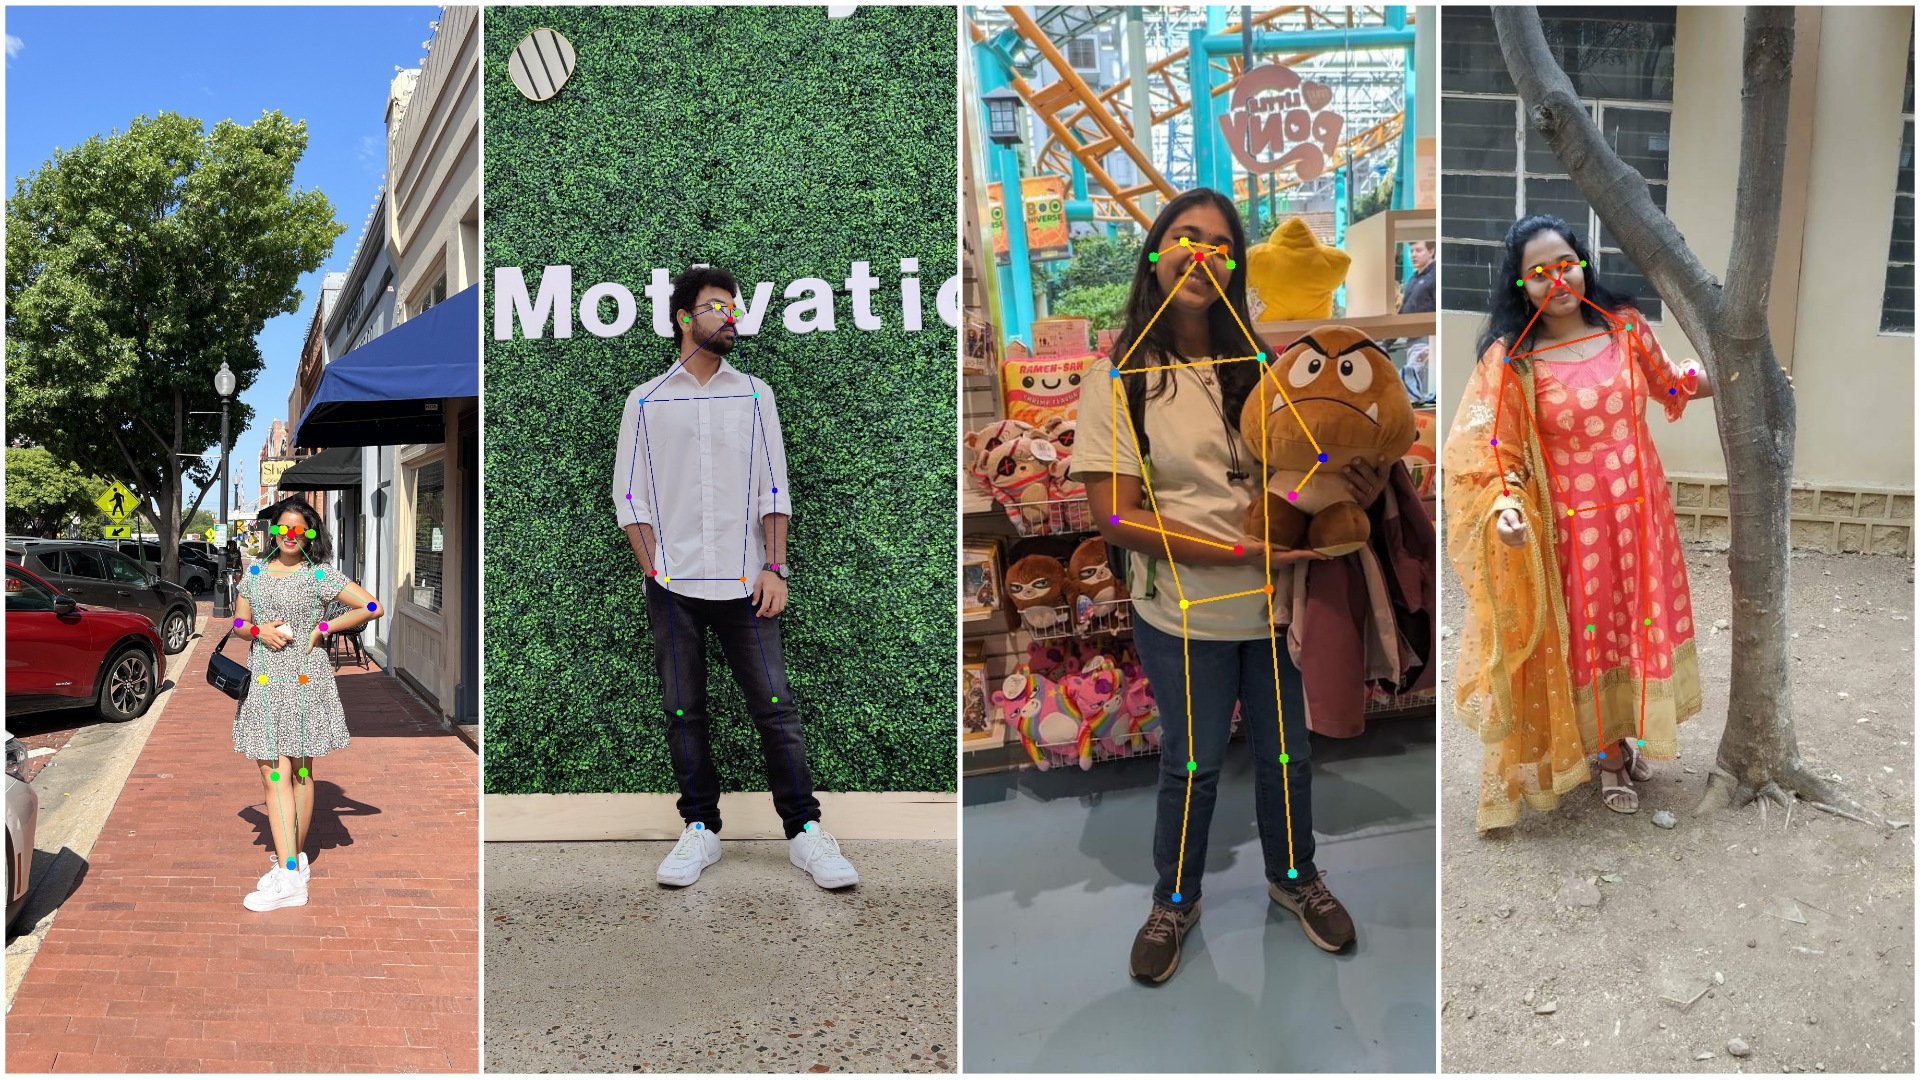
\includegraphics[width=\textwidth]{Image.jpg}
    \caption{Simple HRNet Custom Data Outputs.}
    \label{fig:sub2}
  \end{subfigure}
  \label{fig:group}
\end{figure}

\begin{figure}
  \centering
  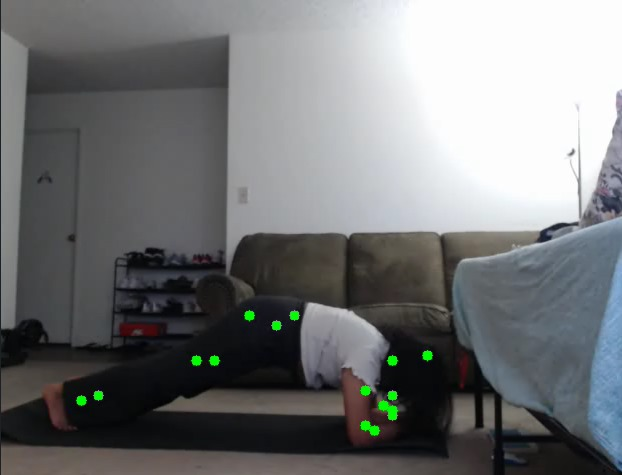
\includegraphics[width=0.7\textwidth]{Raspberrypi_op.jpg}
  \caption{Simple HRNet output from Rapberry Pi on a low resolution web camera}
  \label{fig5}
\end{figure}

\section{Future Steps: Deployment on Raspberry Pi and Feedback System Design}
As we look ahead, the impending phase involves deploying the meticulously trained posture detection model onto a Raspberry Pi, an environment marked by resource constraints compared to conventional computing platforms. This deployment serves as a critical evaluation of the model's efficiency in real-time applications, considering factors such as inference speed and resource consumption. The primary objective is to ascertain that the model's computational demands align with the capabilities of edge devices, thereby enhancing its applicability in scenarios where real-time pose estimation is paramount.

Simultaneously, the future roadmap envisions the evolution of the feedback system. While manual processes currently facilitate corrective feedback, the project aims to automate this process through the creation of a robust dataset and the training of a multi-task learning machine learning model. This advanced model would discern keypoints crucial for distinguishing between correct and incorrect postures, thereby automating the feedback generation process. By visually displaying the correct posture on the screen, the system aims to provide users with immediate and actionable guidance, fostering improved postural habits during various activities.

The cornerstone of these future advancements lies in the keypoint detection model, serving as the core module in the ongoing project. Its role is pivotal not only in accurate posture detection but also in enabling these innovative steps towards deployment on resource-constrained devices and the automation of feedback systems. This strategic integration of machine learning advancements into the project's trajectory reflects a commitment to continuous improvement and adaptation, ensuring the posture detection and correction system remains at the forefront of technological innovation in real-world applications. As we progress, the seamless integration of the model into edge devices and the automation of feedback processes will further solidify the system's practical utility and impact on promoting healthier postural practices.

\begin{figure}
  \centering
  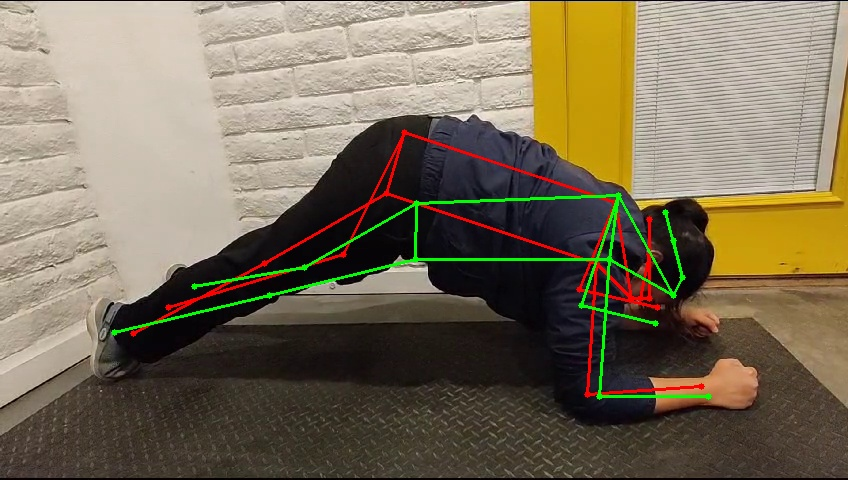
\includegraphics[width=\textwidth]{inference_img1.jpg}
  \caption{Expected visual feedback system.}
  \label{fig6}
\end{figure}


\section*{References}



\medskip


{
\small


[1] Wenqiang Zhang\ \&  Jiemin Fang\ (1995) EfficientPose: Efficient Human Pose Estimation with Neural Architecture Search. In G.\ Tesauro, D.S.\ Touretzky and T.K.\ Leen
(eds.), {\it Advances in Neural Information Processing Systems 7},
pp.\ 609--616. Cambridge, MA: MIT Press.


[2] E. Insafutdinov, L. Pishchulin, B. Andres, M. Andriluka, and
B. Schiele. Deepercut: A deeper, stronger, and faster multiperson pose estimation model. In ECCV, pages 34–50, 2016.


[3] W. Yang, S. Li, W. Ouyang, H. Li, and X. Wang. Learning
feature pyramids for human pose estimation. In ICCV, pages
1290–1299, 2017.

[4] B. Xiao, H. Wu, and Y. Wei. Simple baselines for human
pose estimation and tracking. In ECCV, pages 472–487,
2018. 

[5] J. Wang et al., “Deep High-Resolution Representation Learning for Visual Recognition,” arXiv:1908.07919 [cs], Mar. 2020

[6] Z. Cao, G. Hidalgo, T. Simon, S.-E. Wei, and Y. Sheikh, “OpenPose: Realtime Multi-Person 2D Pose Estimation using Part Affinity Fields,” arXiv:1812.08008 [cs], May 2019

[7] X. Sun, B. Xiao, F. Wei, S. Liang, and Y. Wei, “Integral Human Pose Regression,” arXiv:1711.08229 [cs], Sep. 2018

%%%%%%%%%%%%%%%%%%%%%%%%%%%%%%%%%%%%%%%%%%%%%%%%%%%%%%%%%%%%


\end{document}